%____________________________________________________________________________||
\section{Impact of shape based MC systematics} \label{app:sec_mc_based}

So far we only allowed correlated systematics, e.g. JEC, $b$-tags and more to vary the normalisation only in \MHT. 
In order to test possibly correlated effects on the \MHT variables we test the effect of adding MC based variation on the shape of \MHT.
In particular we are intrested in changes in yield and pull of nuisances. The test have shown now significant deviation. In particularly 


Figures~\ref{fig:mht_shape_axial}-~\ref{fig:mht_shape_scalar} shows the yield obtained with and without shape systematics applied on the \MHT discriminator and
the ratio of both. One sees that no significant difference can be observed. We also tested expected and observed limits with the same result.

\begin{figure}[h!] \centering
  \subfigure{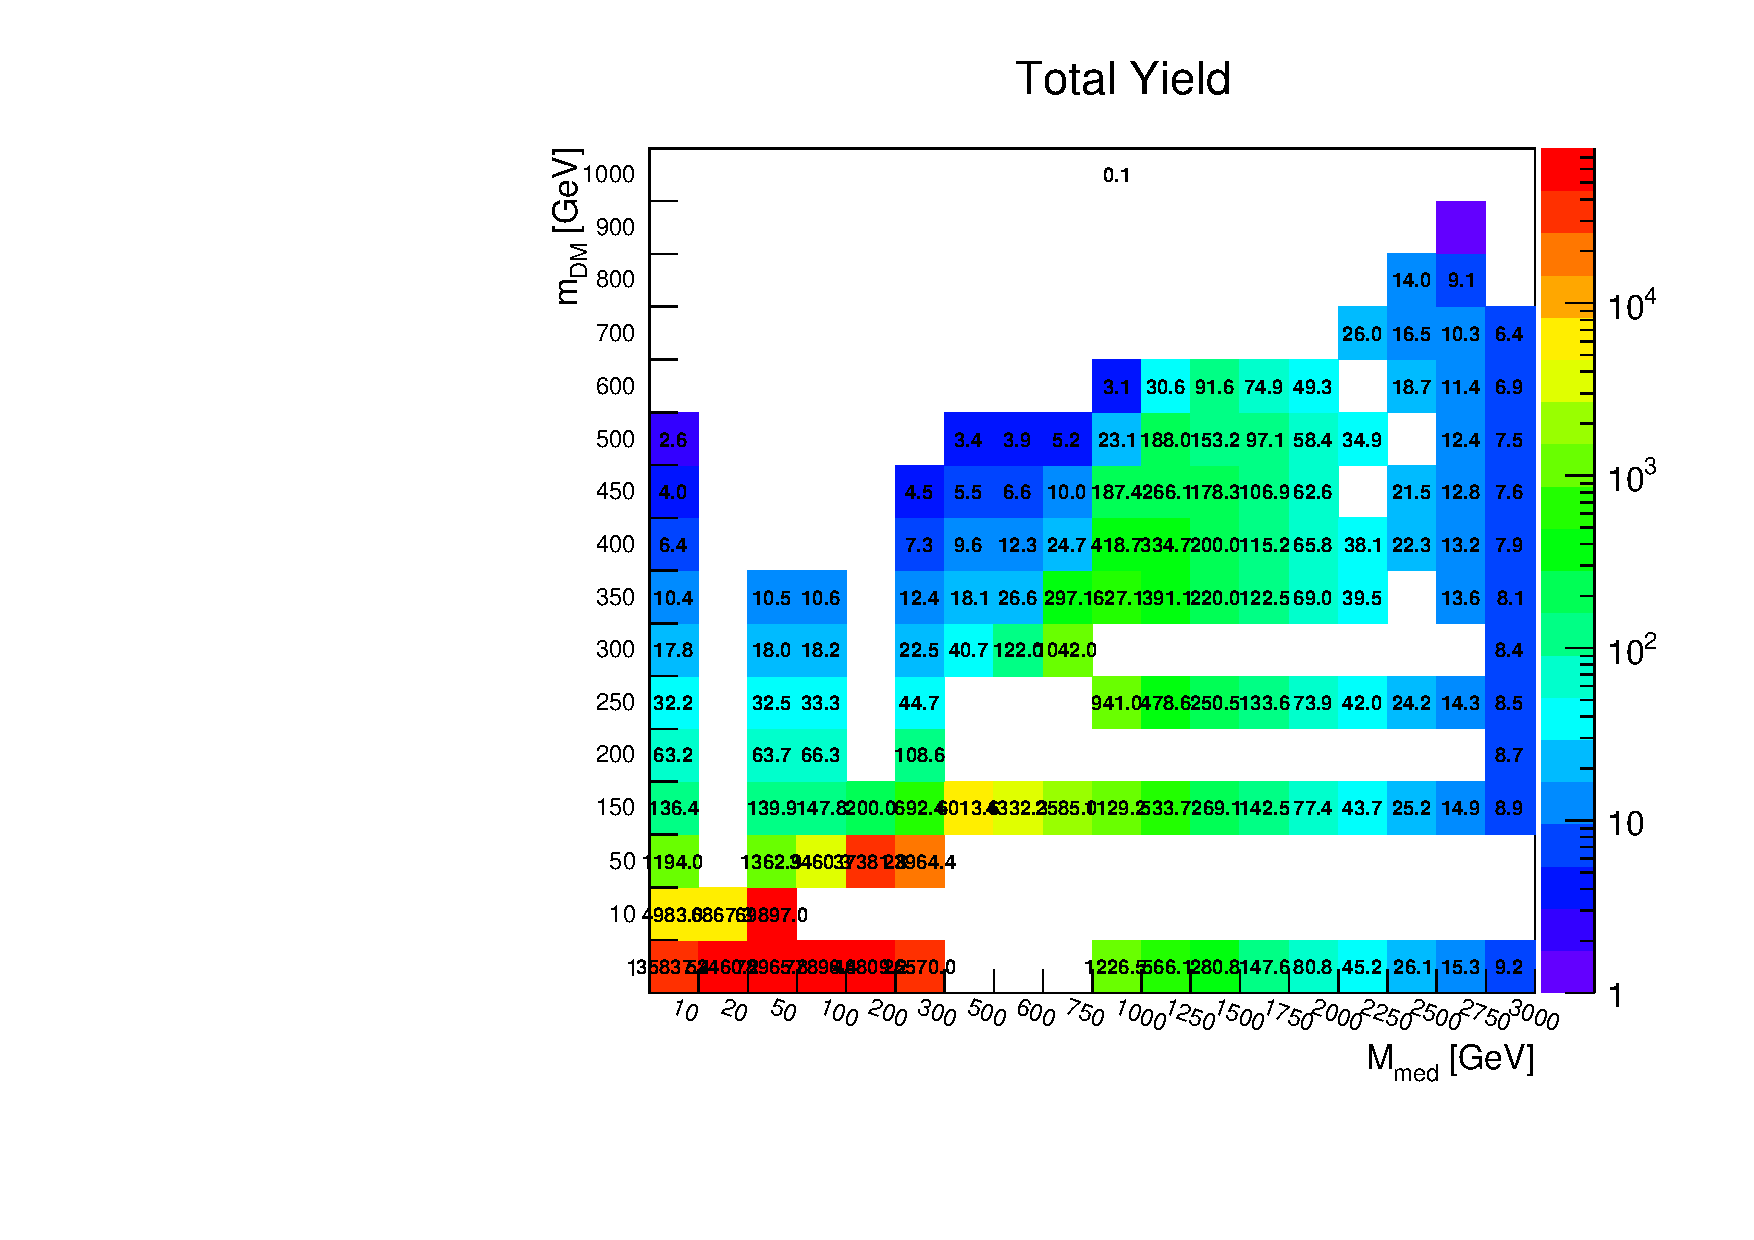
\includegraphics[width=0.35\textwidth]{figures/DMplots/SummaryPlot_ScorpionDMA_xs10_2p2fb_ShapeMCSyst_exp_yldTot.pdf}}
  \subfigure{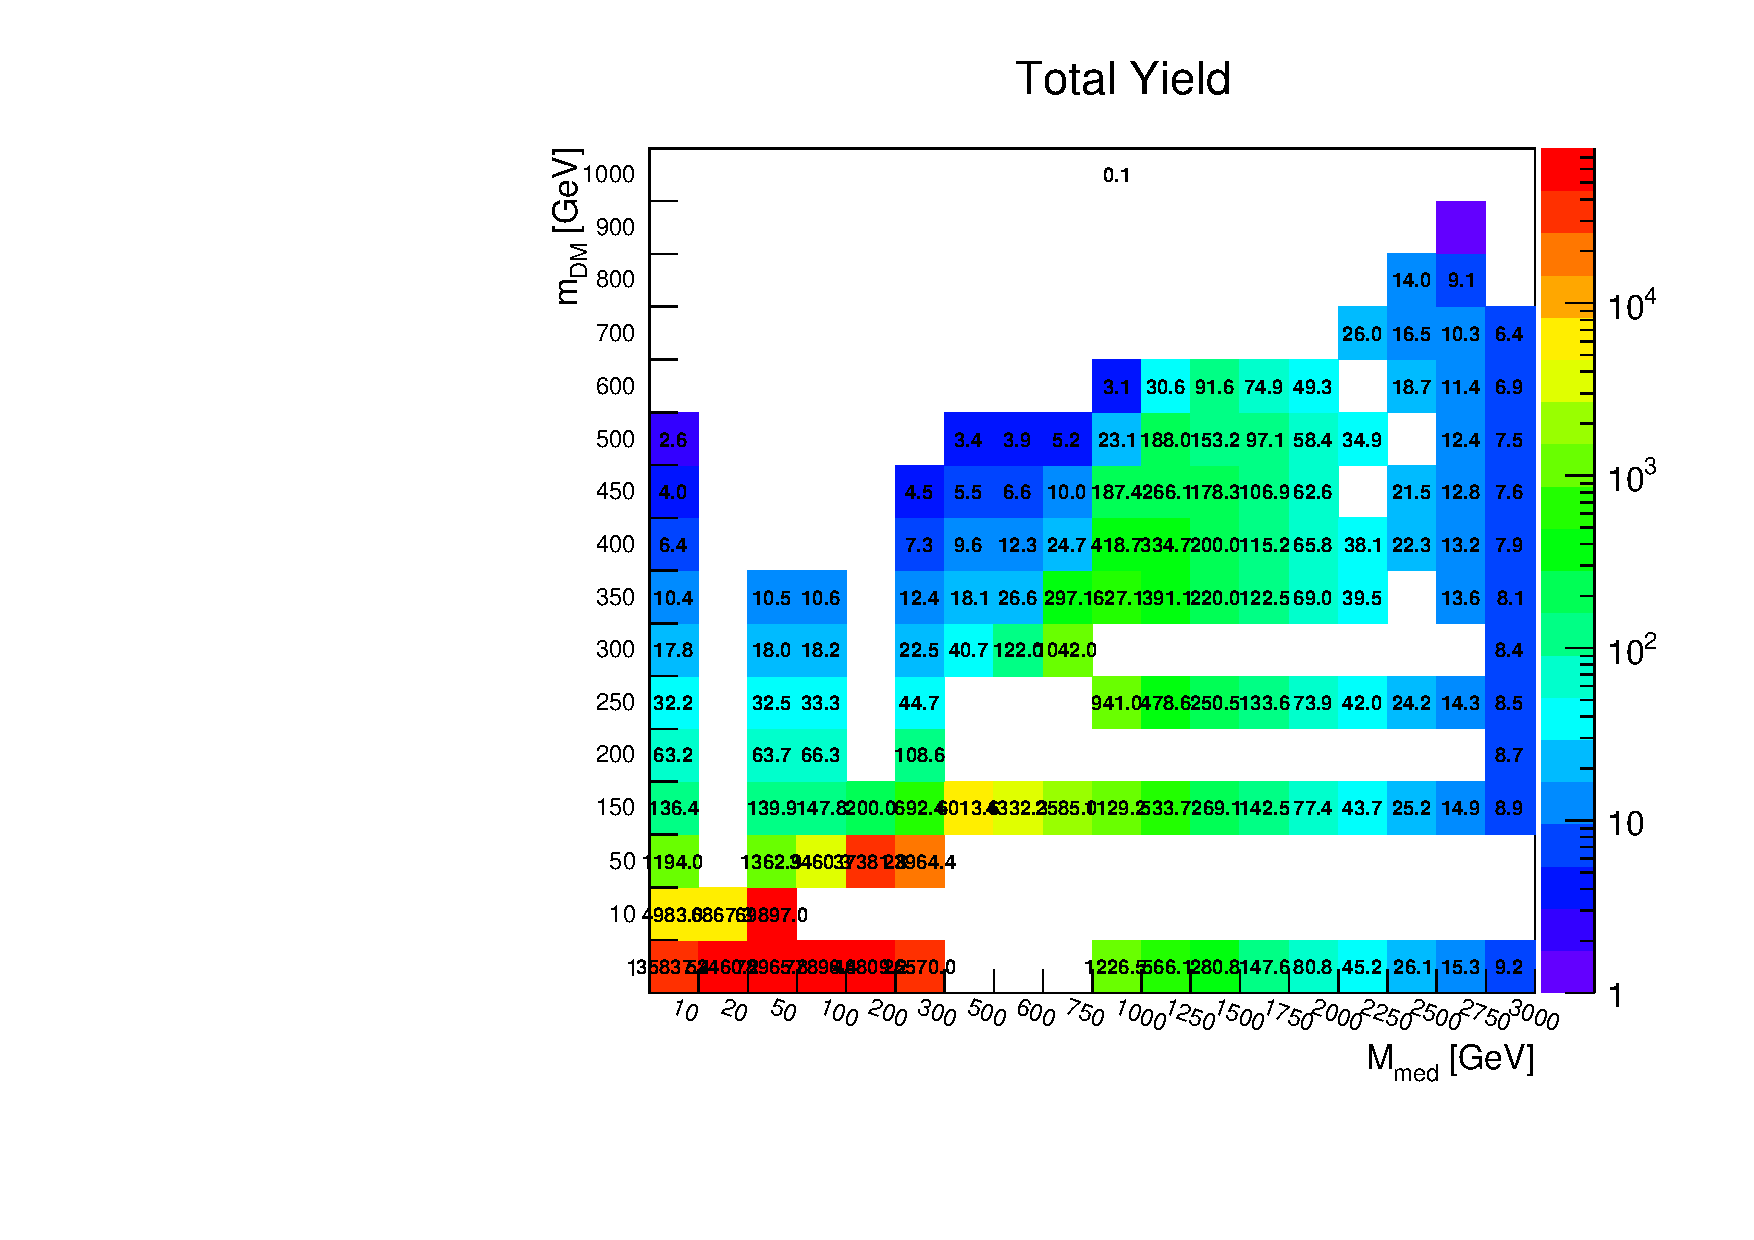
\includegraphics[width=0.35\textwidth]{figures/DMplots/SummaryPlot_ScorpionDMA_xs10_2p2fb_noShapeMCSyst_exp_yldTot.pdf}}
  \subfigure{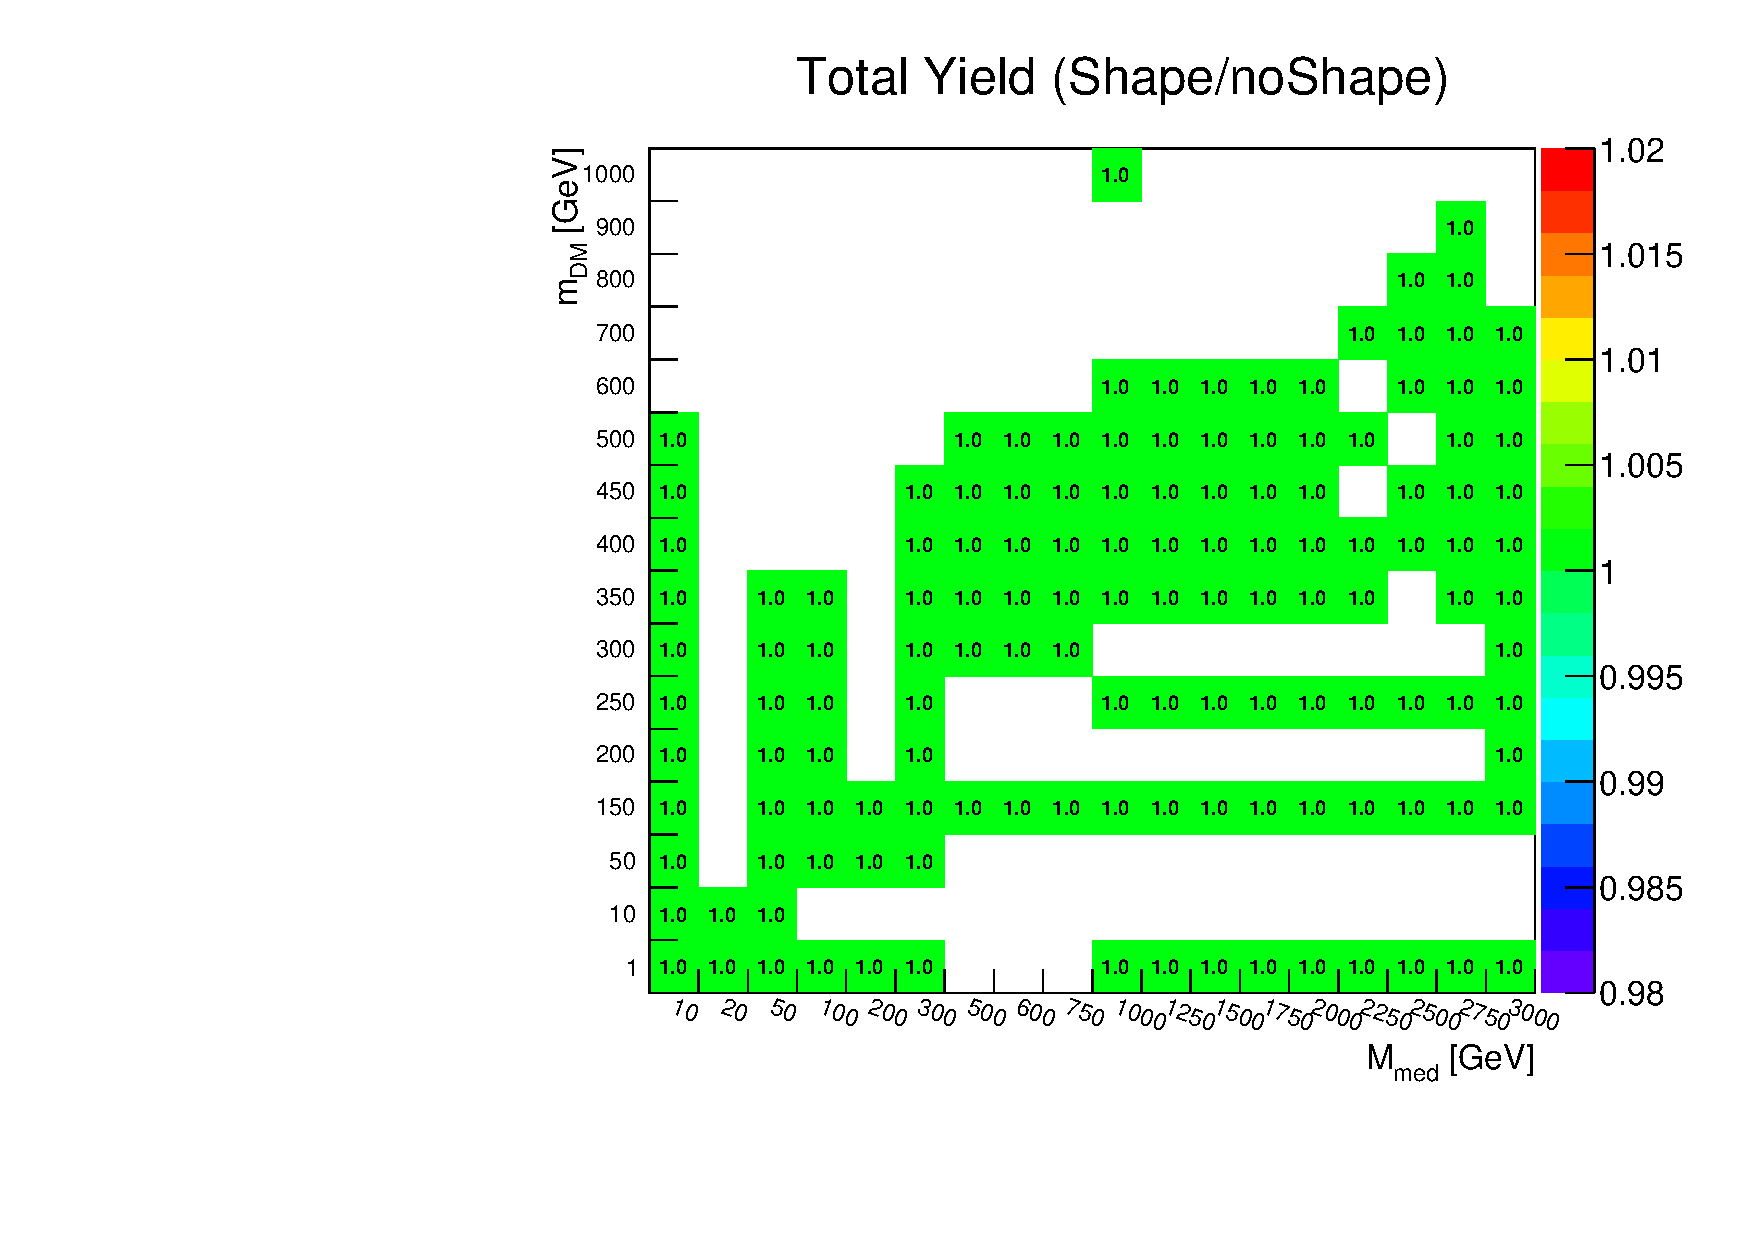
\includegraphics[width=0.35\textwidth]{figures/DMplots/ScorpionDMA_xs10_2p2fb_Shape_DIV_noShape__exp_yldTot.pdf}}
  \caption{Differente between shape systematics considered (left), no shape systematics (middle) and their ratio (right) for axial-vector models.}}
\label{fig:mht_shape_axial} 
\end{figure}



\begin{figure}[h!] \centeringe
  \subfigure{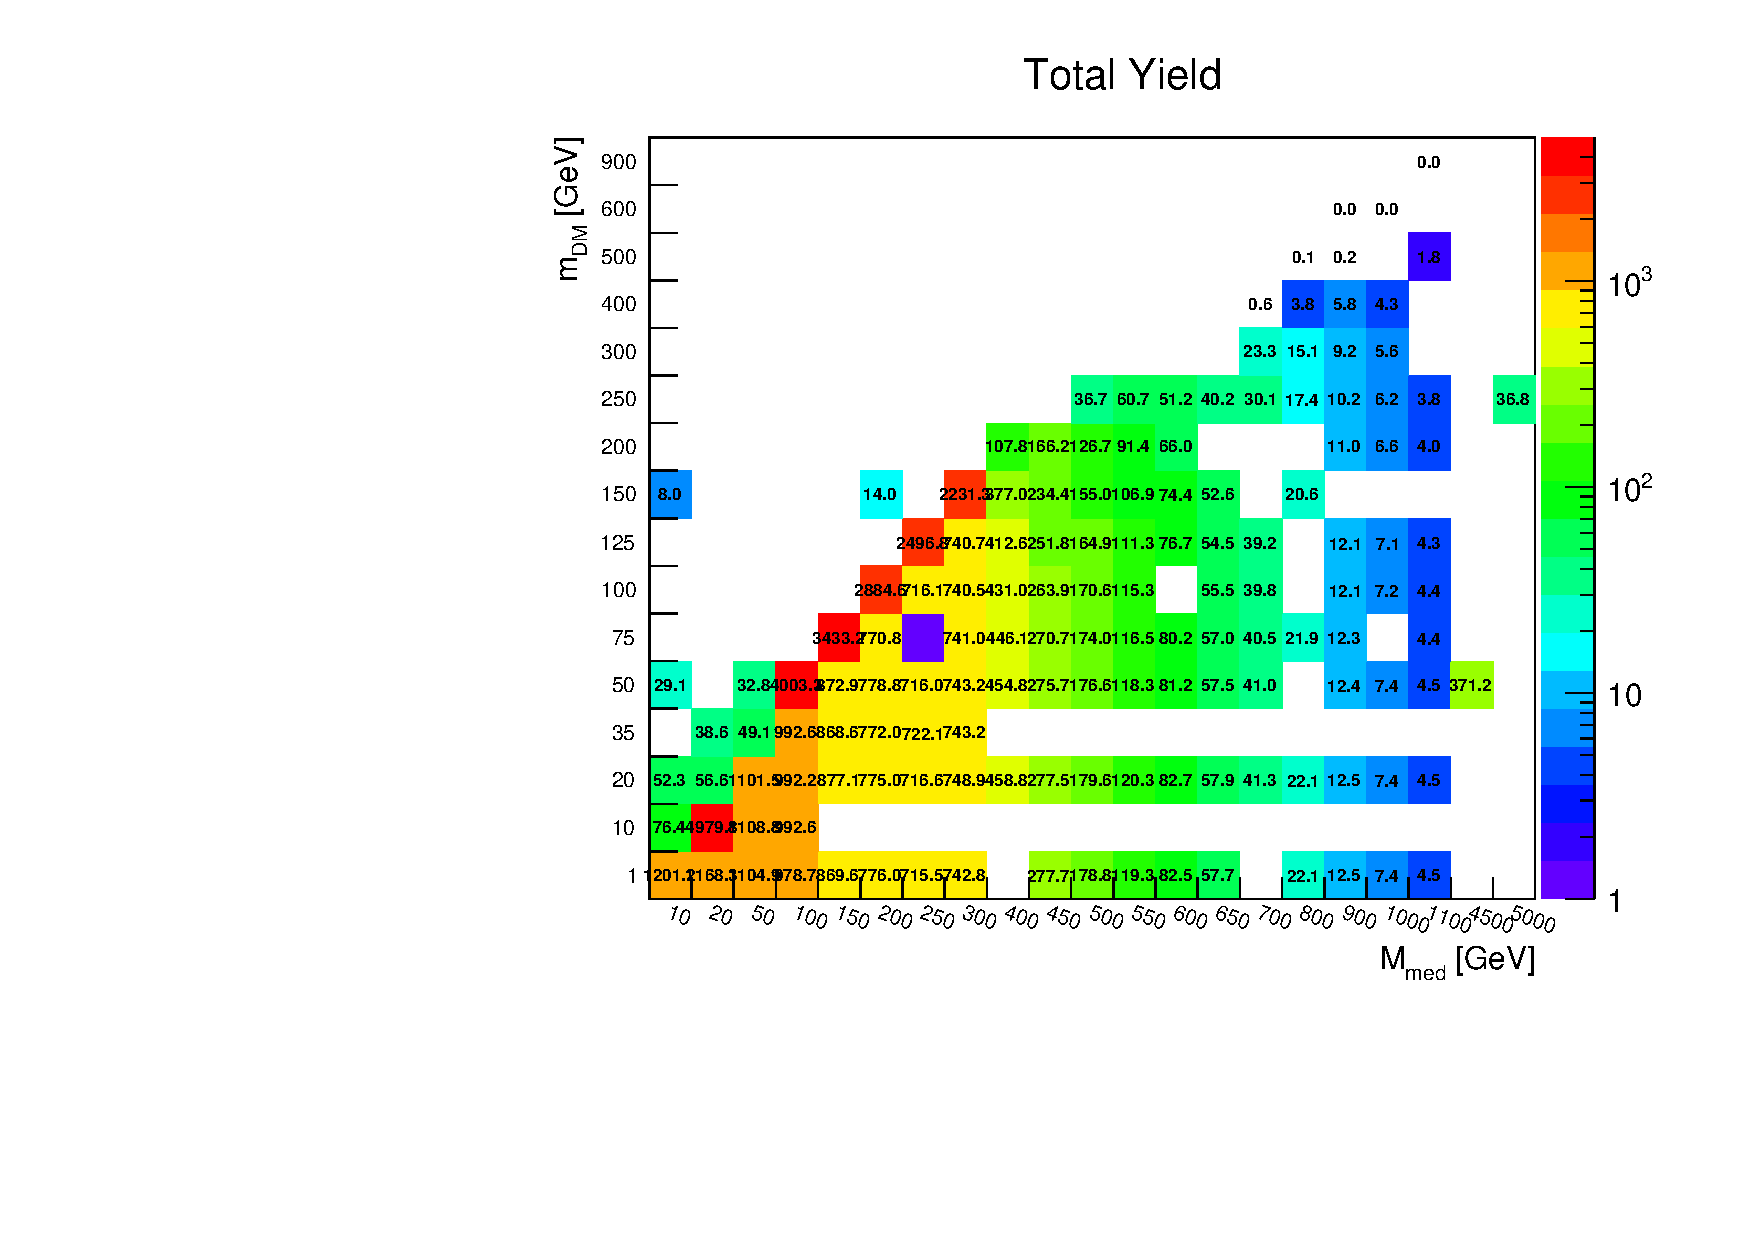
\includegraphics[width=0.35\textwidth]{figures/DMplots/SummaryPlot_ScorpionDMP_xs10_2p2fb_ShapeMCSyst_exp_yldTot.pdf}}
  \subfigure{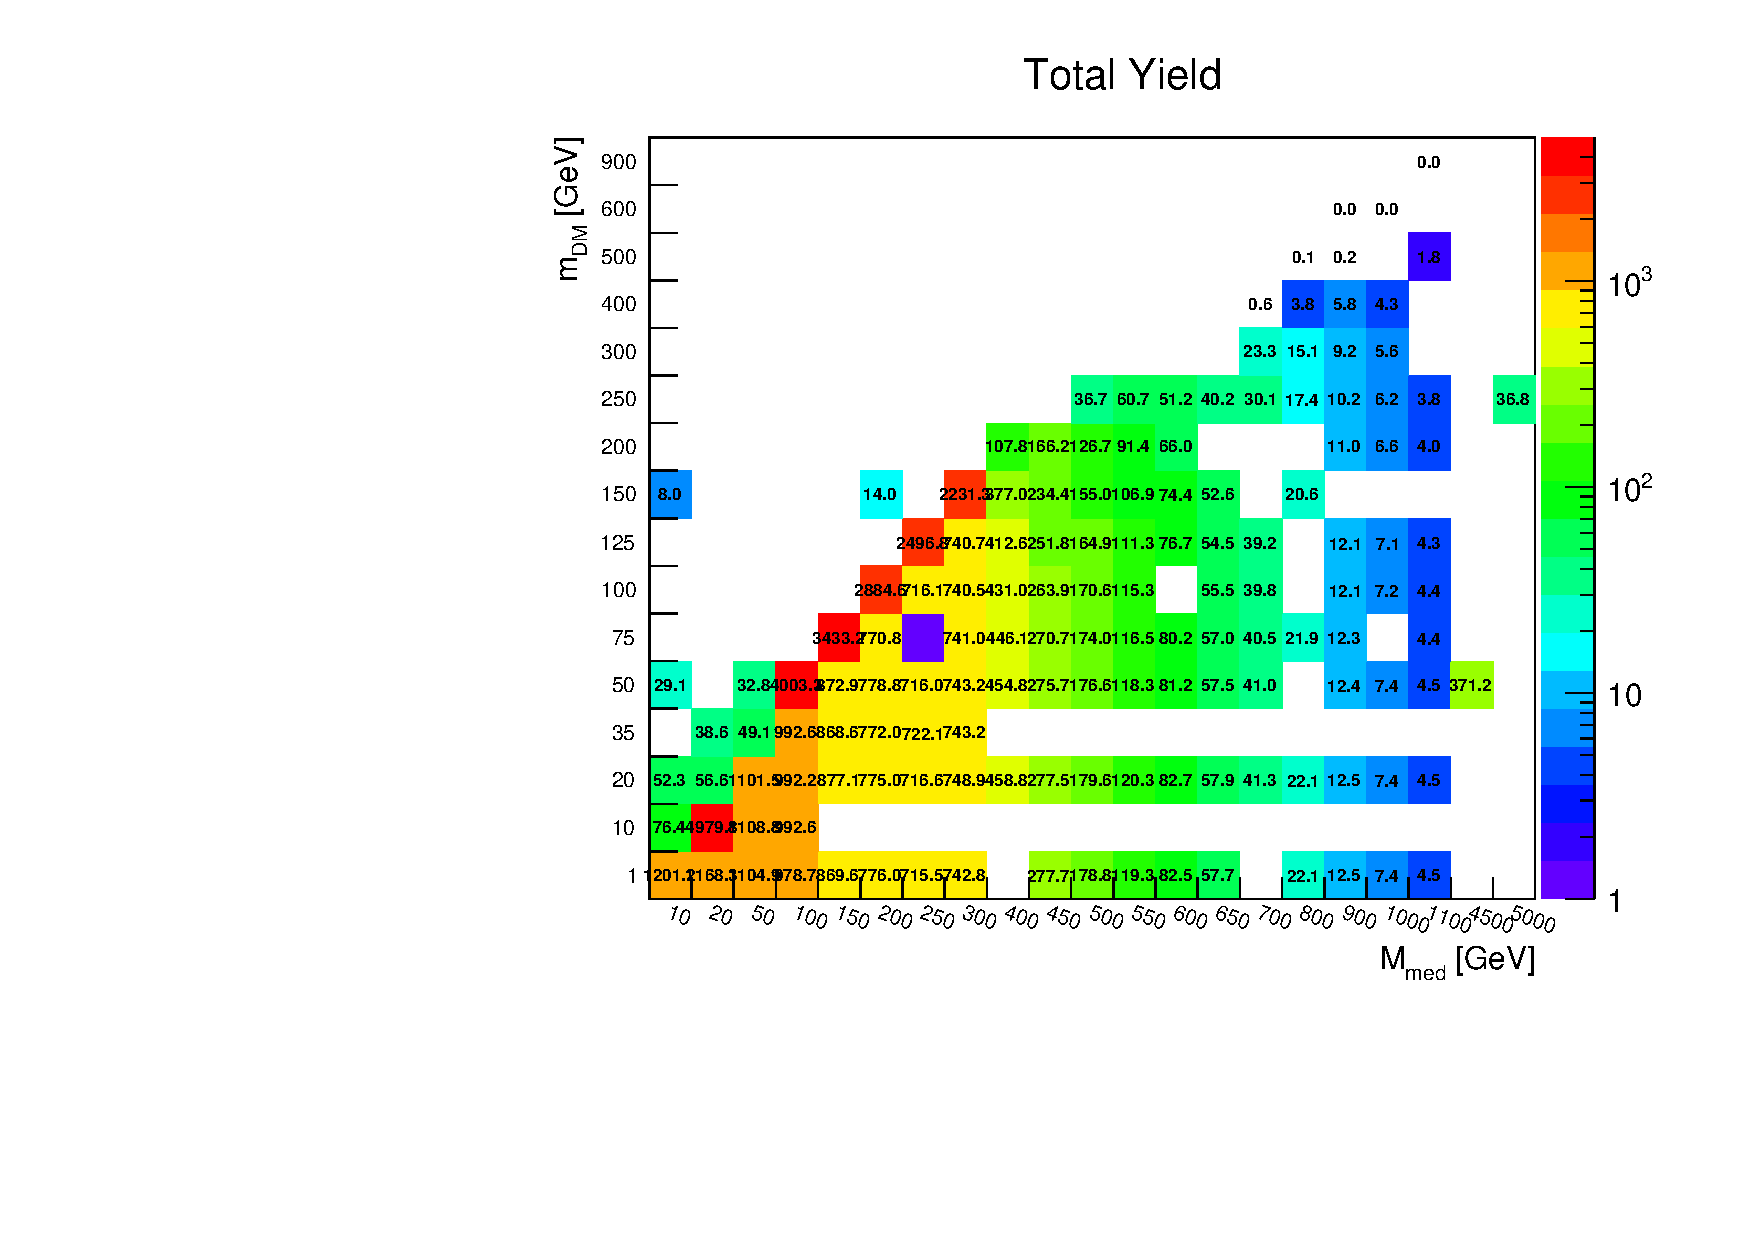
\includegraphics[width=0.35\textwidth]{figures/DMplots/SummaryPlot_ScorpionDMP_xs10_2p2fb_noShapeMCSyst_exp_yldTot.pdf}}
  \subfigure{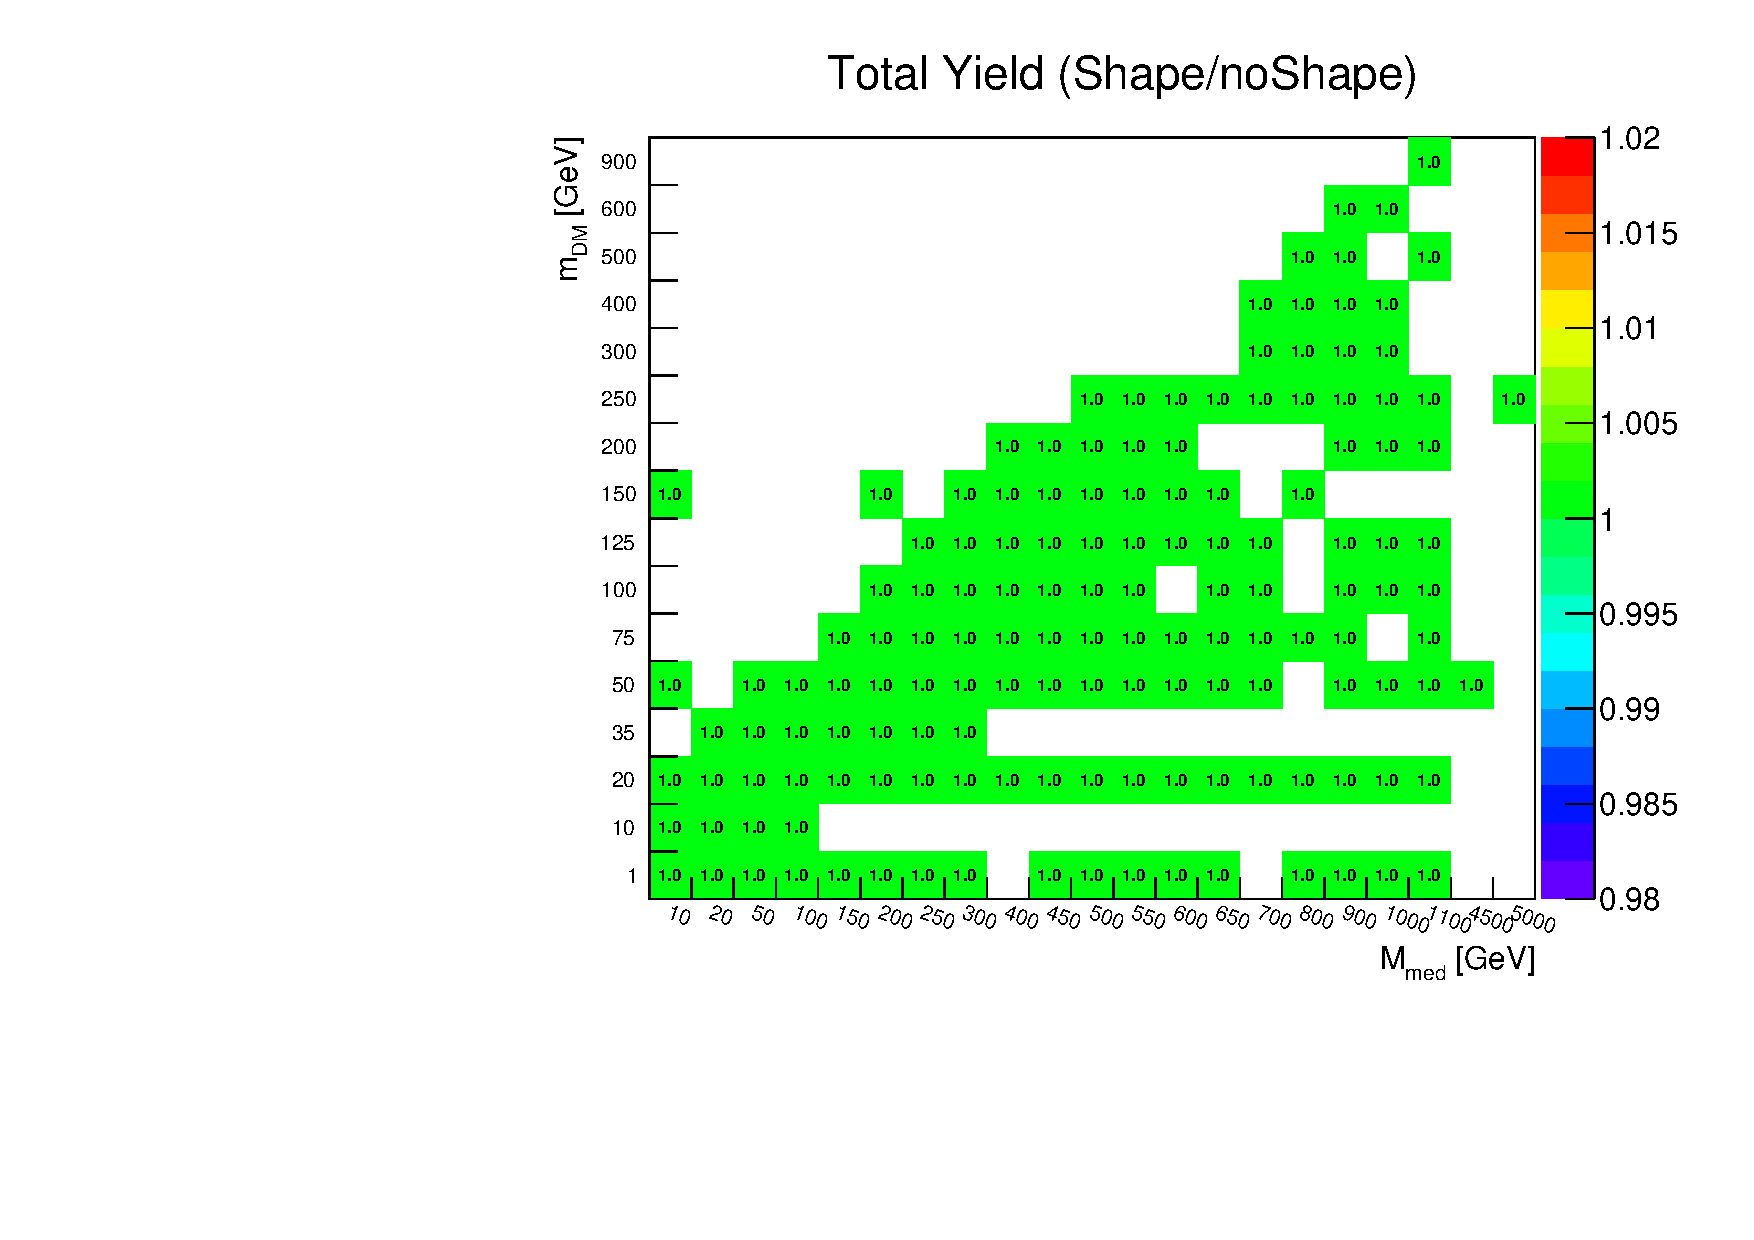
\includegraphics[width=0.35\textwidth]{figures/DMplots/ScorpionDMP_xs10_2p2fb_Shape_DIV_noShape__exp_yldTot.pdf}}
  \caption{Differente between shape systematics considered (left), no shape systematics (middle) and their ratio (right) for scalar models.}}
\label{fig:mht_shape_scalar} 
\end{figure}


